\documentclass{ximera}
%% You can put user macros here
%% However, you cannot make new environments

\listfiles

\graphicspath{{./}{firstExample/}{secondExample/}}

\usepackage{tikz}
\usepackage{tkz-euclide}
\usepackage{tikz-3dplot}
\usepackage{tikz-cd}
\usetikzlibrary{shapes.geometric}
\usetikzlibrary{arrows}
%\usetkzobj{all}
\pgfplotsset{compat=1.13} % prevents compile error.

%\renewcommand{\vec}[1]{\mathbf{#1}}
\renewcommand{\vec}{\mathbf}
\newcommand{\RR}{\mathbb{R}}
\newcommand{\dfn}{\textit}
\newcommand{\dotp}{\cdot}
\newcommand{\id}{\text{id}}
\newcommand\norm[1]{\left\lVert#1\right\rVert}
 
\newtheorem{general}{Generalization}
\newtheorem{initprob}{Exploration Problem}

\tikzstyle geometryDiagrams=[ultra thick,color=blue!50!black]

%\DefineVerbatimEnvironment{octave}{Verbatim}{numbers=left,frame=lines,label=Octave,labelposition=topline}



\usepackage{mathtools}


\title{Curve Fitting} \license{CC BY-NC-SA 4.0}

\begin{document}

\begin{abstract}
\end{abstract}
\maketitle

\begin{onlineOnly}
\section*{Curve Fitting}
\end{onlineOnly}

% \begin{center}
% \begin{tikzpicture}[scale=1]
%   \filldraw[orange](-0.25,3.5)--(0.25,3.5)--(1.5,0)--(-1.5,0)--cycle;
%   \filldraw[orange] (0,0) ellipse (2cm and 1cm);
%   \filldraw[orange] (0,3.5) ellipse (0.25cm and 0.15cm);
% \end{tikzpicture}
 
% UNDER CONSTRUCTION -- COMING SOON
% \end{center}


We know that two points determine a line.  Do you know how many points determine a quadratic function of the form $f(x)=ax^2+bx+c$?  Given any number of points in the plane, is it always possible to find a polynomial function whose graph contains every one of the given points?  To address these questions we will start with an alternative way of finding an equation of a line.

\begin{exploration}\label{exp:curveFitLine}
Consider two points $A(-3, 2)$ and $B(1,-2)$.  We will find a function $f$ whose graph is a line that passes through these points.  We know that $f(x)=ax+b$ for some constants $a$ and $b$.  Because the graph of $f$ passes through $A$ and $B$, we must have the following:
$$\begin{matrix}
      f(-3)&=&a(-3)&+&b&=&2\\
      f(1)&=&a(1)&+&b&=&-2
    \end{matrix}$$
To solve for $a$ and $b$, we need to solve the following matrix equation:
$$\begin{bmatrix}\answer{-3} & \answer{1}\\\answer{1} & \answer{1}\end{bmatrix}\begin{bmatrix}a\\b\end{bmatrix}=\begin{bmatrix}\answer{2}\\\answer{-2}\end{bmatrix}$$
Solving the equation, we find that $a=-1$ and $b=-1$.  This gives us:
$$f(x)=-x-1$$

The GeoGebra interactive below shows two points $A$ and $B$, together with the matrix equation that produces function coefficients for the function whose graph passes through $A$ and $B$.  Drag the points around the plane to see how the matrix equation changes.

\pdfOnly{
Access GeoGebra interactives through the online version of this text at 

\href{https://ximera.osu.edu/oerlinalg}{https://ximera.osu.edu/oerlinalg}.
}

\begin{onlineOnly}
\begin{center}
\geogebra{aupuxe5j}{950}{650}
\end{center}
\end{onlineOnly}

From a purely formal standpoint, we observe that the matrix equation has the form:
$$\begin{matrix}\text{point }A\rightarrow\\\text{point }B\rightarrow\end{matrix}\begin{bmatrix}x\text{-coordinate} & 1\\x\text{-coordinate} & 1\end{bmatrix}\begin{bmatrix}a\\b\end{bmatrix}=\begin{bmatrix}y\text{-coordinate}\\y\text{-coordinate}\end{bmatrix}$$
where each row corresponds to one point.
\end{exploration}

Now we are ready to move to quadratic, and higher degree polynomial functions.

Linear function in Exploration \ref{exp:curveFitLine} had two unknown coefficients that we needed to find in order to determine the function. Two points gave us a system of two equations and two unknowns.

A quadratic polynomial function, whose graph is a parabola, is given by:
$$f(x)=ax^2+bx+c$$
Three unknown coefficients will require three points to determine them.

\begin{exploration}\label{exp:curveFitParabola}
We will find a quadratic function of the form $f(x)=ax^2+bx+c$ whose graph passes through $A(-2,2)$, $B(0, -1)$ and $C(1, 5)$.
To do this, we need to find coefficients $a$, $b$ and $c$ such that
$$\begin{matrix}f(-2)&=&a(-2)^2&+&b(-2)&+&c&=&2\\f(0)&=&a(0)^2&+&b(0)&+&c&=&-1\\f(1)&=&a(1)^2&+&b(1)&+&c&=&5\end{matrix}$$

The following GeoGebra interactive shows points $A$, $B$, and $C$, together with the matrix equation, and its solution.

\pdfOnly{
Access GeoGebra interactives through the online version of this text at 

\href{https://ximera.osu.edu/oerlinalg}{https://ximera.osu.edu/oerlinalg}.
}

\begin{onlineOnly}
\begin{center}
\geogebra{m6mbcykf}{950}{650}
\end{center}
\end{onlineOnly}

Drag the points around the plane to observe changes in the coefficient matrix.  Think geometrically to find locations of $A$, $B$ and $C$ such that
\begin{itemize}
    \item $a=b=0$; $c\neq 0$.
    \item $a=0$; $b, c\neq 0$.
\end{itemize}

Observe the structure of the matrix equation.
$$\begin{matrix}\text{point }A\rightarrow\\\text{point }B\rightarrow\\\text{point }C\rightarrow\end{matrix}\begin{bmatrix}(x\text{-coordinate})^2&x\text{-coordinate} & 1\\(x\text{-coordinate})^2&x\text{-coordinate} & 1\\(x\text{-coordinate})^2&x\text{-coordinate} & 1\end{bmatrix}\begin{bmatrix}a\\b\\c\end{bmatrix}=\begin{bmatrix}y\text{-coordinate}\\y\text{-coordinate}\\y\text{-coordinate}\end{bmatrix}$$
\end{exploration}

In general (provided that no one point lies directly above another), given $n$ points, we can always find an $(n-1)$-degree polynomial function whose graph contains every one of the given points.  To find such a polynomial function, given by $f(x)=a_{n-1}x^{n-1}+\dots +a_1x+a_0$, we need to solve a system of $n$ equations with $n$ unknowns which translates into the following matrix equation.

\begin{equation}\label{eq:matEq}\begin{bmatrix}\vdots&\vdots &\vdots &\vdots\\(x\text{-coordinate})^{n-1}&\dots &x\text{-coordinate} &1\\\vdots&\vdots &\vdots &\vdots\end{bmatrix}\begin{bmatrix}a_{n-1}\\\vdots\\a_1\\a_0\end{bmatrix}=\begin{bmatrix}\vdots\\y\text{-coordinate}\\\vdots\end{bmatrix}\end{equation}

In Practice Problems \ref{prob:systemProblems1} and \ref{prob:systemProblems2} you will show that the matrix equation in (\ref{eq:matEq}) has a unique solution if and only if no two of the given points share an $x$-coordinate.

\subsection*{Using Technology}
Throughout this section we have omitted the tedious process of solving matrix equations.  It is useful to practice solving smaller  matrix equations by hand, but for larger matrices, we can use technology.  Below is the Octave code that can be used to find the solution to Exploration \ref{exp:curveFitParabola}.  You will be able to modify this code to solve some of the practice problems.

To use Octave, go to the \href{https://sagecell.sagemath.org/}{Sage Math Cell Webpage}, copy the code below into the cell, select OCTAVE as the language, and press EVALUATE.

\begin{verbatim}
% Define the coefficient matrix
A=[4 -2 1;0 0 1;1 1 1];
% Define vector b
b=[2;-1;5];
% We can find the solution in two ways
% Method 1: ans1=A^(-1)b  
ans1=inv(A)*b
% Method 2
ans2=A\b
% If A is invertible, both methods produce the same result.
\end{verbatim}

\subsection*{On the Dangers of Overfitting}
It is exciting to know that we can fit a function to a set of data points, but before we get carried away fitting a 299-degree polynomial function to 300 points, let's consider the following situation.

In the GeoGebra interactive below, you can see that points $A$ - $F$ form a somewhat linear pattern.  A linear model can be used to describe these points.  Click on the ``Display linear model" check-box to see the trend line.  (You will learn how to find such models in \href{https://ximera.osu.edu/oerlinalg/LinearAlgebra/RTH-0030/main}{Least-Squares Approximation}).  You can see that even though the line does not pass through any of the given points, it fits the overall pattern of the points and can be used to estimate the $y$-coordinates of other points whose $x$-coordinates fall within the limits of the scatter plot.

It might be tempting to think that we can find a better model by finding a $5^{th}$-degree polynomial function whose graph contains every one of the six points.  Click on the ``Display 5th degree poly model" check-box to see the alternative model.  Can this model be successfully used to make predictions?

Try moving individual points around to see how their placement affects the line and the curve.

\pdfOnly{
Access GeoGebra interactives through the online version of this text at 

\href{https://ximera.osu.edu/oerlinalg}{https://ximera.osu.edu/oerlinalg}.
}

\begin{onlineOnly}
\begin{center}
\geogebra{z2qhxkmm}{950}{650}
\end{center}
\end{onlineOnly}

Any modeling process which insists on fitting the existing data points exactly, at the risk of failing to predict future observations, is referred to as \emph{overfitting}.  While sometimes it is beneficial to have a curve that passes through specific points, more often it is the trend, not the individual instances, that we try to capture.  We will return to this topic in   \href{https://ximera.osu.edu/oerlinalg/LinearAlgebra/RTH-0030/main}{Least-Squares Approximation}.

\section*{Practice Problems}
\begin{problem}
In each case, find a polynomial function of an appropriate degree that passes through the given points.

\begin{problem}\label{prob:polyFit1}
    $$(-3,0), (2, -2), (-1,1)$$
 $$f(x)=\answer{-0.3x^2-0.7x+0.6}$$
 Plot the graph of $f$ in the Desmos window below.

 \begin{onlineOnly}
\begin{center}
\desmos{aba3troiar}{950}{650}
\end{center}
\end{onlineOnly}
\end{problem}

\begin{problem}\label{prob:polyFit2}
$$(0,4), (-2, 2), (-1,1), (0.5, 1)$$
$$g(x)=\answer{-3.2x^3-7.6x^2-1.4x+4}$$

 Plot the graph of $g$ in the Desmos window below.
     \begin{onlineOnly}
\begin{center}
\desmos{a0fvniud45}{950}{650}
\end{center}
\end{onlineOnly}
\end{problem}
    
\end{problem}

\begin{problem}\label{prob:systemProblems1}
Two GeoGebra screenshots are shown below:

\begin{center}
        \begin{tikzpicture}
\node[inner sep=0pt, anchor=base] (p1) at (0,0)
  {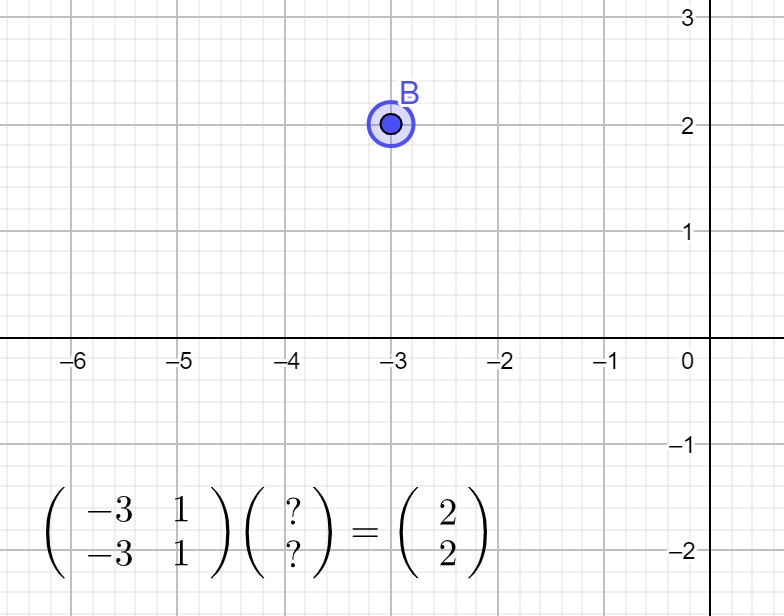
\includegraphics[height=50mm]{pointsCoincide.jpg}};
         \end{tikzpicture}
  \quad\quad
   \begin{tikzpicture}[scale=2]
 \node[inner sep=0pt, anchor=base]  (p2) at (0,0)
  {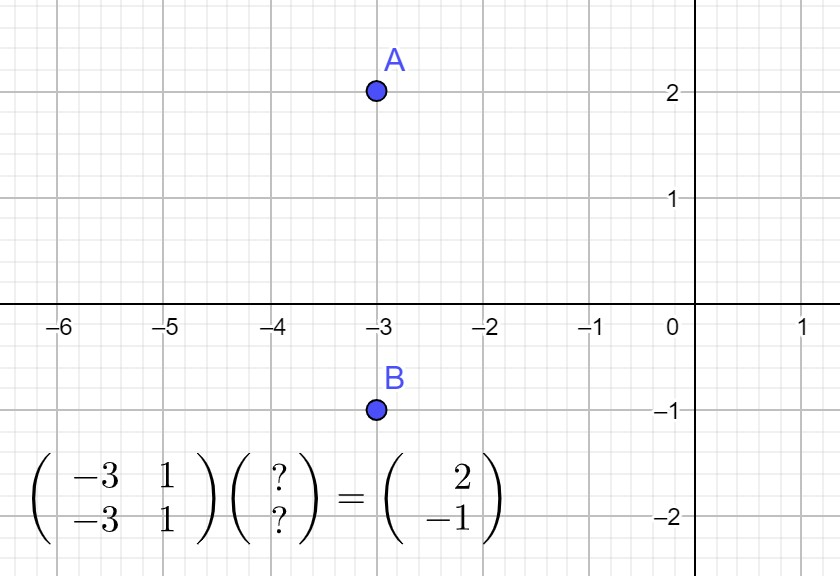
\includegraphics[height=50mm]{verticalPoints.jpg}};
    \end{tikzpicture}
    \end{center}

%     \begin{image}
%          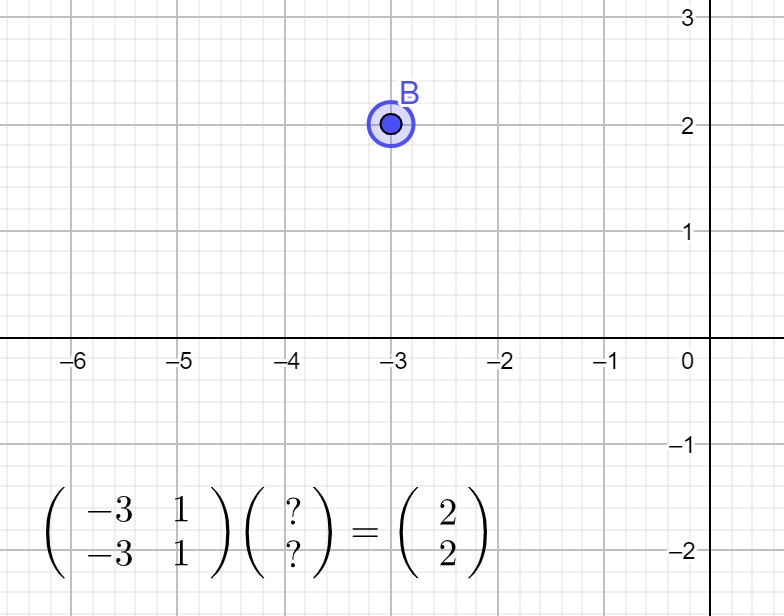
\includegraphics[height=1.5in]{pointsCoincide.jpg}\quad
%          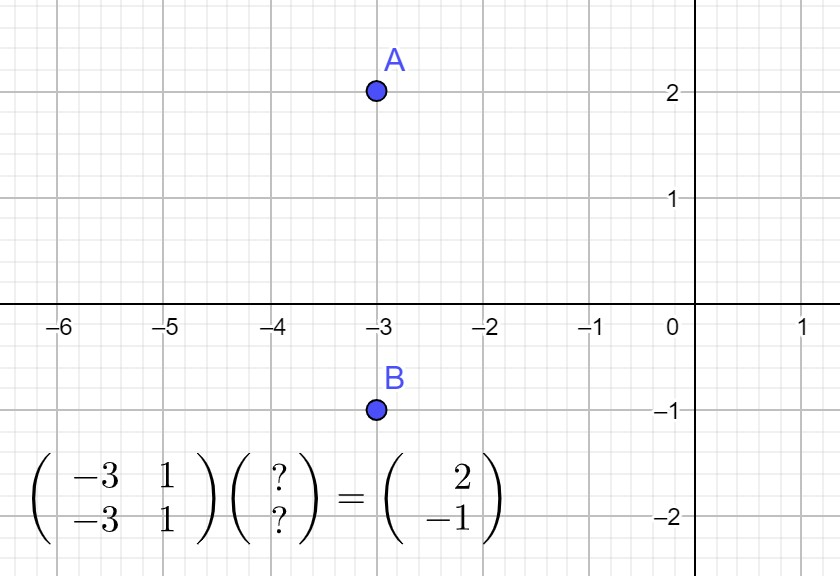
\includegraphics[height=1.5in]{verticalPoints.jpg}
% \end{image}
In the first screenshot, points $A$ and $B$ coincide.  In the second screenshot, point $A$ is located directly above point $B$. 
In both cases, GeoGebra failed to produce a linear function whose graph passes through $A$ and $B$.

Based on what you know about functions and geometry, explain why the process fails for these two examples. How do your observations correspond to what happens from an algebraic standpoint?

\begin{multipleChoice}
    \choice{Both systems are inconsistent.}
    \choice{The first system is inconsistent, the second has infinitely many solutions.}
    \choice{Both systems have infinitely many solutions.}
    \choice[correct]{The first system has infinitely many solutions, the second system is inconsistent.}
\end{multipleChoice}
\end{problem}

\begin{problem}\label{prob:systemProblems2}
Prove that equation (\ref{eq:matEq}) has a unique solution if and only if no two given points share an $x$-coordinate.
\begin{hint}
    Show that the rows of the matrix are linearly independent if and only if no two given points share an $x$-coordinate.
\end{hint}
Under what circumstances is a solution not unique?  Under what circumstances does a solution not exist?
\end{problem}




\end{document}